%!TEX program = xelatex
%!TEX options = --shell-escape
\documentclass[10pt,a4paper]{article}
\usepackage[cache=false]{minted}
\usepackage[utf8]{inputenc}
\usepackage{ctex}
\usepackage{assignpkg}
\usepackage{amsmath}
\usepackage{amssymb}

\usepackage{tikz}
\usetikzlibrary{fpu}

\studentIds{202XX80XXXXXXXX}{}
\studentNames{XXX}{}

\assignmentNumber{4}

\date{\today}

\begin{document}

\makecover
\section*{1 DES第一轮的计算}
第1轮的输出为
FFFFFFFF
61545920。
附录A,B为原始代码。若要得到结果,需运行$\$ruby\ DES.rb$。

\section*{2 AES初始化轮和第一轮的计算}
附录C,D为原始代码。若要得到结果,需运行$\$ruby\ AES.rb$。

\begin{itemize}
    \item[] (1)State最初的内容

    \begin{tabular}{cccc}
    00 & 04 & 08 & 0C \\
    01 & 05 & 09 & 0D \\
    02 & 06 & 0A & 0E \\
    03 & 07 & 0B & 0F \\    
    \end{tabular}
    \item[] (2)初始化轮密钥加密后的值

    \begin{tabular}{cccc}
        01 & 05 & 09 & 0D \\
        00 & 04 & 08 & 0C \\
        03 & 07 & 0B & 0F \\
        02 & 06 & 0A & 0E \\
    \end{tabular}

    \item[] (3)字节替换后的结果

    \begin{tabular}{cccc}
        7C & 6B & 01 & D7 \\
        63 & F2 & 30 & FE \\
        7B & C5 & 2B & 76 \\
        77 & 6F & 67 & AB \\
    \end{tabular}

    \item[] (4)行移位后的结果

    \begin{tabular}{cccc}
        7C & 6B & 01 & D7 \\
        F2 & 30 & FE & 63 \\
        2B & 76 & 7B & C5 \\
        AB & 77 & 6F & 67 \\
    \end{tabular}
    
    \item[] (5)列混淆之后的结果

    \begin{tabular}{cccc}
        75 & 87 & 0F & B2 \\
        55 & E6 & 04 & 22 \\
        3E & 2E & B8 & 8C \\
        10 & 15 & 58 & 0A \\
    \end{tabular}

    \item[] (6)第一轮使用的轮密钥
    
    \begin{tabular}{cccc}
        7F & 7E & 7F & 7E \\
        7D & 7C & 7D & 7C \\
        7D & 7C & 7D & 7C \\
        7D & 7C & 7D & 7C \\
    \end{tabular}


\end{itemize}

\section*{3 DES中与Sbox有关偏差的计算}
根据课件,$X_2$应当是S盒的6位输入的次高位比特,而$Y_1,Y_2,Y_3,Y_4$为输出的4个比特。


\begin{tabular}{ccc}
 $Sbox_i$ & 该随机变量等于0的次数 & 偏差 \\
0 & 14 & -0.281250 \\
1 & 20 & -0.187500 \\
2 & 42 & 0.156250 \\
3 & 40 & 0.125000 \\
4 & 12 & -0.312500 \\
5 & 42 & 0.156250 \\
6 & 18 & -0.218750 \\
7 & 16 & -0.250000 \\
\end{tabular}

附代码:
\begin{minted}[tabsize=8,obeytabs,showtabs]{ruby}
require "./init.rb"
puts " 第i个S盒 & 该随机变量等于0的次数 & 偏差 \\\\"
total = 64.0
8.times do |i|
    count = 0.0
    4.times do |j|
        16.times do |k|
            count_ones = (Sbox[i][j][k]*2 + k/8).to_s(2).scan("1").length
            if count_ones % 2 == 0
                count += 1
            end
        end
    end
    puts "%d & %d & %f \\\\" %[i, count, count/total - 0.5]
end
\end{minted}
\section*{4 AES的差分特征}

\begin{figure}[htbp]
\centering
    \tikzstyle{register}=[draw, thick, minimum width=0.6cm, minimum height=0.6cm, 
                                    draw=black!100,
                                    fill=pink!20
                                    ]
    \tikzstyle{XOR}=[circle,thick,minimum size=0.5cm,
                                    draw=magenta!80,
                                    fill=pink!20]

\begin{tikzpicture}[thick]
    \begin{scope}
        \foreach \j in {0,...,3}{
            \foreach \i in {0,...,3}{
                \node (vector\j\i) [register] at (0.6 * \i+5, -0.6 * \j + 3) {};
            }
        }
        \node (vector02) [register] at (vector02) {$f$};
        \node (vector13) [register] at (vector13) {$g$};
        \node (vector20) [register] at (vector20) {$h$};
        \node (vector31) [register] at (vector31) {$i$};
        \foreach \k in {0,...,4}{
            \foreach \j in {0,...,3}{
                \foreach \i in {0,...,3}{
                    \node (vector\k\j\i) [register] at (0.6 * \i + \k * 3.2, -0.6 * \j) {};
                }
            }
        }
        %\node (vector123) [register] at (vector123) {f};
        \node at ([yshift=0.7cm]vector01) {$Round\ 1$};
        \node (delta_p) at ([yshift=-0.7cm]vector31) {Plaintext :$P$(明文的差分)};
        \node () at ([yshift=-0.7cm]vector031) {state :$S_1^{I}$};
        \node () at ([yshift=-0.7cm]vector131) {state :$S_1^{SB}$};
        \node () at ([yshift=-0.7cm]vector231) {state :$S_1^{SR}$};
        \node () at ([yshift=-0.7cm]vector331) {state :$S_1^{MC}$};
        \node () at ([yshift=-0.7cm]vector431) {state :$S_1^{AK}$};
        %\draw[-latex] 
        \node (vector002) [register] at (vector002) {$f$};
        \node (vector013) [register] at (vector013) {$g$};
        \node (vector020) [register] at (vector020) {$h$};
        \node (vector031) [register] at (vector031) {$i$};
        \begin{scriptsize}
        \node [register] at (vector102) {$Da$};
        \node [register] at (vector113) {$Ba$};
        \node [register] at (vector120) {$Ea$};
        \node [register] at (vector131) {$9a$};        
        \end{scriptsize}

        \draw[->,thick] (vector002) to [in = 90, out = 90] node {差分转移} (vector102) ;
        \draw[->,thick] (vector013) to [in = 90, out = 90] (vector113) ;
        \draw[->,thick] (vector020) to [in = 90, out = 90] (vector120) ;
        \draw[->,thick] (vector031) to [in = 90, out = 90] (vector131) ;
        \begin{scriptsize}
        \node at (vector202) {$Da$};
        \node at (vector212) {$Ba$};
        \node at (vector222) {$Ea$};
        \node at (vector232) {$9a$};        
        \end{scriptsize}
        \node at (vector322) {$a$};
        \node at (vector422) {$a$};
    \end{scope}

\end{tikzpicture}
\begin{tikzpicture}
    \node at (0,-2) {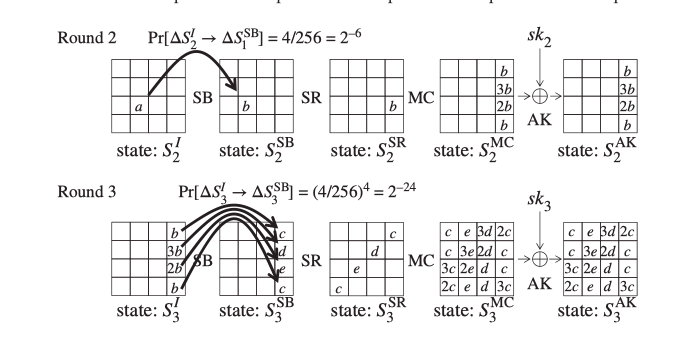
\includegraphics[width=14cm,height=7cm]{round.png}};
\end{tikzpicture}
\end{figure}

如上图所示,前三轮的一个可能的查分特征寻找方法如上图所示,明文一开始的差分如第一个矩阵所示,我们不指出其具体的差分值是多少,我们仅以字母表示该处的差分。
为了构造一个查分,我们首先确定第一轮末的一个差分,假定其是$a$,设$a$能差分转移到$b$,可以向前和向后推到这个差分转移向第一轮传播和向后面两轮传播的情况。如图所示,具体不再阐述。其中二三轮的查分推导截图来自《Security of Block Ciphers From Algorithm Design to Hardware Implementation-Wiley 2015》
\section*{5 偏差}
记$X_1 \oplus X_2$为随机变量$X_1 \oplus X_2$,$X_2\oplus X_3$为随机变量$X_2 \oplus X_3$,
则
$X_1 \oplus X_2$与$X_2\oplus X_3$互相独立$\iff P(X_1 \oplus X_2=i,X_2 \oplus X_3=j) = P(X_1 \oplus X_2=i)P(X_2 \oplus X_3=j),\ i,j \in \{0,1\}\iff $



$$
\left\{\begin{aligned}
P(X_1 \oplus X_2=0,X_2 \oplus X_3=0) = P(X_1 \oplus X_2=0)P(X_2 \oplus X_3=0)\\
P(X_1 \oplus X_2=0,X_2 \oplus X_3=1) = P(X_1 \oplus X_2=0)P(X_2 \oplus X_3=1)\\
P(X_1 \oplus X_2=1,X_2 \oplus X_3=0) = P(X_1 \oplus X_2=1)P(X_2 \oplus X_3=0)\\
P(X_1 \oplus X_2=1,X_2 \oplus X_3=1) = P(X_1 \oplus X_2=1)P(X_2 \oplus X_3=1)
\end{aligned}\right.
$$
$\iff$
$$
\left\{\begin{aligned}
(\frac{1}{2}+\epsilon_1)(\frac{1}{2}+\epsilon_2)(\frac{1}{2}+\epsilon_3) + (\frac{1}{2}-\epsilon_1)(\frac{1}{2}-\epsilon_2)(\frac{1}{2}-\epsilon_3) = (\frac{1}{2}+2\epsilon_1\epsilon_2)(\frac{1}{2}+2\epsilon_2\epsilon_3)\\
(\frac{1}{2}+\epsilon_1)(\frac{1}{2}+\epsilon_2)(\frac{1}{2}-\epsilon_3) + (\frac{1}{2}-\epsilon_1)(\frac{1}{2}-\epsilon_2)(\frac{1}{2}+\epsilon_3) = (\frac{1}{2}+2\epsilon_1\epsilon_2)(\frac{1}{2}-2\epsilon_2\epsilon_3)\\
(\frac{1}{2}+\epsilon_1)(\frac{1}{2}-\epsilon_2)(\frac{1}{2}-\epsilon_3) + (\frac{1}{2}-\epsilon_1)(\frac{1}{2}+\epsilon_2)(\frac{1}{2}+\epsilon_3) = (\frac{1}{2}-2\epsilon_1\epsilon_2)(\frac{1}{2}+2\epsilon_2\epsilon_3)\\
(\frac{1}{2}-\epsilon_1)(\frac{1}{2}+\epsilon_2)(\frac{1}{2}-\epsilon_3) + (\frac{1}{2}+\epsilon_1)(\frac{1}{2}-\epsilon_2)(\frac{1}{2}+\epsilon_3) = (\frac{1}{2}-2\epsilon_1\epsilon_2)(\frac{1}{2}-2\epsilon_2\epsilon_3)
\end{aligned}\right.
$$
上述四式化简后均得到$4\epsilon_1\epsilon_2^2\epsilon_3=\epsilon_1\epsilon_3$。

$4\epsilon_1\epsilon_2^2\epsilon_3=\epsilon_1\epsilon_3 \iff (4\epsilon_2^2-1)\epsilon_1\epsilon_2=0 \iff \epsilon_1 = 0\ or\ \epsilon_3=0\ or\ \epsilon_2=\pm\frac{1}{2}$
\section*{6 RSA加密}
\begin{itemize}
\item[] (1)
    因为公钥$e=17$,$n = p\times q = 77,\ \phi(n) = 6 \times 10 = 60$,私钥$d=e^{-1} \mod \phi(n) = 53$,故密文$c=m^d \mod n = 8 ^ {53} \mod 77 = 50$
\item[] (2)
    若采用蒙哥马利算法,则由53的二进制展开$(110101)_2$,根据蒙哥马利算法,从次高位开始至最低位,若该位为1,则进行一次模平方运算和一次模乘运算,即两次模乘运算;若该位为0,则进行一次模平方运算(一次模乘)。次高位至最低位共有3个1和2个0,故共需$3\times2+2\times1=8$次模乘运算。
\end{itemize}

\section*{7 RSA解密}
公开密钥$(e,n)=(5, 35)$,密文$c$为10,求明文$m$,意即已知$m^5 \mod 35 = 10$,求$m$。
而只要求出加密所用的私钥$d$即可。

因为$d,e$满足$de \mod \phi(n) = 1$,$n=5\times7,\ \phi(n) = 4\times6 = 24$,根据欧几里得算法,可计算$d=5$,故明文$m=c^5\mod 35 = 10^5 \mod 35 = 5$。

\appendix
 % \renewcommand{\appendixname}{Appendix~\Alph{section}}
 \section{$init.rb$}
\begin{minted}{ruby}
# in all of the matrixs, the index starts with 1

# the initial permutaion of plaintext
IP = [
    58,50,42,34,26,18,10,2,60,52,44,36,28,20,12,4,
    62,54,46,38,30,22,14,6,64,56,48,40,32,24,16,8,
    57,49,41,33,25,17,9,1,59,51,43,35,27,19,11,3,
    61,53,45,37,29,21,13,5,63,55,47,39,31,23,15,7
]

# the permutation matrix of key extension
PC_1 = [
    57, 49, 41, 33, 25, 17, 9,
    1, 58, 50, 42, 34, 26, 18,
    10, 2, 59, 51, 43, 35, 27,
    19, 11, 3, 60, 52, 44, 36,
    63, 55, 47, 39, 31, 23, 15,
    7, 62, 54, 46, 38, 30, 22,
    14, 6, 61, 53, 45, 37, 29,
    21, 13, 5, 28, 20, 12, 4
]

PC_2 = [
    14, 17, 11, 24,  1, 5,
    3, 28, 15,  6, 21, 10,
    23, 19, 12,  4, 26,  8,
    16,  7, 27, 20, 13,  2,
    41, 52, 31, 37, 47, 55,
    30, 40, 51, 45, 33, 48,
    44, 49, 39, 56, 34, 53,
    46, 42, 50, 36, 29, 32
]

# the eight sbox used between AddDey and Pbox permutation
Sbox = [
    [
        [14,4,13,1,2,15,11,8,3,10,6,12,5,9,0,7],
        [0,15,7,4,14,2,13,1,10,6,12,11,9,5,3,8],
        [4,1,14,8,13,6,2,11,15,12,9,7,3,10,5,0],
        [15,12,8,2,4,9,1,7,5,11,3,14,10,0,6,13],
    ],
    [
        [15,1,8,14,6,11,3,4,9,7,2,13,12,0,5,10],
        [3,13,4,7,15,2,8,14,12,0,1,10,6,9,11,5],
        [0,14,7,11,10,4,13,1,5,8,12,6,9,3,2,15],
        [13,8,10,1,3,15,4,2,11,6,7,12,0,5,14,9],
    ],
    [
        [10,0,9,14,6,3,15,5,1,13,12,7,11,4,2,8],
        [13,7,0,9,3,4,6,10,2,8,5,14,12,11,15,1],
        [13,6,4,9,8,15,3,0,11,1,2,12,5,10,14,7],
        [1,10,13,0,6,9,8,7,4,15,14,3,11,5,2,12],
    ],
    [
        [7,13,14,3,0,6,9,10,1,2,8,5,11,12,4,15],
        [13,8,11,5,6,15,0,3,4,7,2,12,1,10,14,9],
        [10,6,9,0,12,11,7,13,15,1,3,14,5,2,8,4],
        [3,15,0,6,10,1,13,8,9,4,5,11,12,7,2,14],
    ],
    [
        [2,12,4,1,7,10,11,6,8,5,3,15,13,0,14,9],
        [14,11,2,12,4,7,13,1,5,0,15,10,3,9,8,6],
        [4,2,1,11,10,13,7,8,15,9,12,5,6,3,0,14],
        [11,8,12,7,1,14,2,13,6,15,0,9,10,4,5,3],
    ],
    [
        [12,1,10,15,9,2,6,8,0,13,3,4,14,7,5,11],
        [10,15,4,2,7,12,9,5,6,1,13,14,0,11,3,8],
        [9,14,15,5,2,8,12,3,7,0,4,10,1,13,11,6],
        [4,3,2,12,9,5,15,10,11,14,1,7,6,0,8,13],
    ],
    [
        [4,11,2,14,15,0,8,13,3,12,9,7,5,10,6,1],
        [13,0,11,7,4,9,1,10,14,3,5,12,2,15,8,6],
        [1,4,11,13,12,3,7,14,10,15,6,8,0,5,9,2],
        [6,11,13,8,1,4,10,7,9,5,0,15,14,2,3,12],
    ],
    [
        [13,2,8,4,6,15,11,1,10,9,3,14,5,0,12,7],
        [1,15,13,8,10,3,7,4,12,5,6,11,0,14,9,2],
        [7,11,4,1,9,12,14,2,0,6,10,13,15,3,5,8],
        [2,1,14,7,4,10,8,13,15,12,9,0,3,5,6,11],
    ]
]

# the permutation that extends the right 32 bits of last round to 48 bits
E = [
    32,1,2,3,4,5,4,5,6,7,8,9,
    8,9,10,11,12,13,12,13,14,15,16,17,
    16,17,18,19,20,21,20,21,22,23,24,25,
    24,25,26,27,28,29,28,29,30,31,32,1
]

# the permutation after the Sbox
P = [
    16,7,20,21,29,12,28,17,
    1,15,23,26,5,18,31,10,
    2,8,24,14,32,27,3,9,
    19,13,30,6,22,11,4,25
]

\end{minted}
 \section{$DES.rb$}
  \begin{minted}{ruby}
require "./init.rb"

class ConvertArray
    #convert array to binary string, delimited by a space
    def self.toBinary(input)
        input.each_slice(4) . map . inject("") {|sum, s| sum << (s . join . to_s + " ")}
    end
    #convert array to hex string, delimited by a space
    def self.toHex(input)
        x = input.each_slice(4) . map . inject("") {|sum, s| sum << s . join . to_s}
        "%08X" % x.to_i(2)
    end
end

class Bignum
    def hex_to_binary_arr
        bin_len = self.to_s(16) . length * 4
        format = "%#{bin_len}d"
        sprintf(format, self.to_s(2)) . split("") . map(&:to_i)
    end
end

class Fixnum
    def hex_to_binary_arr
        bin_len = self.to_s(16) . length * 4
        format = "%#{bin_len}d"
        sprintf(format, self.to_s(2)) . split("") . map(&:to_i)
    end
end

def printHex(input)
    puts "#{ConvertArray.toHex(input)}" 
end

def printBin(input)
    puts "#{ConvertArray.toBinary(input)}"
end

class DES
    def AddCheckBits(key)
        key_bits = key.hex_to_binary_arr 
        # key_bits = @key.hex_to_binary_arr
        i = 8
        # extend key to 64 bits
        until i < 1 do
            sum = 0
            j = 7
            until j < 1 do
                sum += key_bits[7*i-j]
                j = j - 1
            end
            key_bits[7*i, 0] = sum % 2
            i = i - 1
        end
        key_bits
    end

    def permutation(count, origin_arr, permute_arr)
        out_arr = []
        count.times do |i|
            out_arr[i] = origin_arr[permute_arr[i] - 1]
        end
        out_arr
    end

    def shift(c_in, d_in)
        if @round == 1 || @round == 2 || @round == 9 || @round == 16
            c_out = @c_in[1..27] + [@c_in[0]]
            d_out = @d_in[1..27] + [@d_in[0]]
        else
            c_out = @c_in[2..27] + @c_in[0..1]
            d_out = @d_in[2..27] + @d_in[0..1]
        end
        return c_out, d_out
    end

    def round_key(c_in, d_in)
        #@c_in, @d_in = shift()
        tmp = @c_in + @d_in
        roundkey = permutation(48, tmp, PC_2)
    end

    def getPlaintex_IP
        @plaintext
    end

    def getKey
        @key
    end

    def round_function
        @c_in, @d_in = shift(@c_in, @d_in) 
        roundkey = round_key(@c_in, @d_in)

        l = @r
        r_e = permutation(48, @r, E)
        sbox_in_array = r_e.zip(roundkey).map { |x,y| x^y }
        sbox_8_in = sbox_in_array . each_slice(6) . map . inject([]) { |sum, s| sum << s.join.to_i(2) }
        sbox_outputs = []

        8.times do |i|
            tmp = sbox_8_in[i]
            j = tmp / 32 * 2 +  (tmp % 2)
            k = (tmp % 32) / 2
            sbox_outputs[i] = Sbox[i][j][k]
        end

        sb_out = sbox_outputs.each.map.inject([]) { |sum, s| sum << sprintf("%04d", s.to_s(2)).split("")}

        sb_out = sb_out.flatten.each.map(&:to_i)
        
        sbox_outputs_P = permutation(32, sb_out, P)
        r = sbox_outputs_P.zip(@l).map { |x,y| x^y }
        printHex(l)
        printHex(r)
        @l, @r = l, r
        @round = @round + 1
    end

    def sixteen_rounds
        15.times do |i|
            puts "第%d轮的输出" % (i+2)
            round_function
        end
    end

    def initialize(key, plaintext)
        if key.to_s(16) .length == 14
            @key = AddCheckBits(key)
        else
            @key = key.hex_to_binary_arr
        end
        @key = permutation(56, @key, PC_1)
        @plaintext = permutation(64, plaintext.hex_to_binary_arr, IP)
        @round = 1
        @c_in = @key[0..27]
        @d_in = @key[28..55]
        @l = @plaintext[0..31]
        @r = @plaintext[32..63]
    end
end

key = 0x55555555555555
plaintext = 0xFEFEFEFEFEFEFEFE

des = DES.new(key, plaintext)
puts "第1轮的输出"
des.round_function()

des.sixteen_rounds()
  \end{minted}
\section{$AESSbox.rb$}
\begin{minted}{ruby}
AesBox=[
    [0x63, 0x7c, 0x77, 0x7b, 0xf2, 0x6b, 0x6f, 0xc5, 0x30, 0x01, 0x67, 0x2b, 0xfe, 0xd7, 0xab, 0x76], 
    [0xca, 0x82, 0xc9, 0x7d, 0xfa, 0x59, 0x47, 0xf0, 0xad, 0xd4, 0xa2, 0xaf, 0x9c, 0xa4, 0x72, 0xc0], 
    [0xb7, 0xfd, 0x93, 0x26, 0x36, 0x3f, 0xf7, 0xcc, 0x34, 0xa5, 0xe5, 0xf1, 0x71, 0xd8, 0x31, 0x15],
    [0x04, 0xc7, 0x23, 0xc3, 0x18, 0x96, 0x05, 0x9a, 0x07, 0x12, 0x80, 0xe2, 0xeb, 0x27, 0xb2, 0x75], 
    [0x09, 0x83, 0x2c, 0x1a, 0x1b, 0x6e, 0x5a, 0xa0, 0x52, 0x3b, 0xd6, 0xb3, 0x29, 0xe3, 0x2f, 0x84], 
    [0x53, 0xd1, 0x00, 0xed, 0x20, 0xfc, 0xb1, 0x5b, 0x6a, 0xcb, 0xbe, 0x39, 0x4a, 0x4c, 0x58, 0xcf],
    [0xd0, 0xef, 0xaa, 0xfb, 0x43, 0x4d, 0x33, 0x85, 0x45, 0xf9, 0x02, 0x7f, 0x50, 0x3c, 0x9f, 0xa8],
    [0x51, 0xa3, 0x40, 0x8f, 0x92, 0x9d, 0x38, 0xf5, 0xbc, 0xb6, 0xda, 0x21, 0x10, 0xff, 0xf3, 0xd2],
    [0xcd, 0x0c, 0x13, 0xec, 0x5f, 0x97, 0x44, 0x17, 0xc4, 0xa7, 0x7e, 0x3d, 0x64, 0x5d, 0x19, 0x73],
    [0x60, 0x81, 0x4f, 0xdc, 0x22, 0x2a, 0x90, 0x88, 0x46, 0xee, 0xb8, 0x14, 0xde, 0x5e, 0x0b, 0xdb], 
    [0xe0, 0x32, 0x3a, 0x0a, 0x49, 0x06, 0x24, 0x5c, 0xc2, 0xd3, 0xac, 0x62, 0x91, 0x95, 0xe4, 0x79], 
    [0xe7, 0xc8, 0x37, 0x6d, 0x8d, 0xd5, 0x4e, 0xa9, 0x6c, 0x56, 0xf4, 0xea, 0x65, 0x7a, 0xae, 0x08], 
    [0xba, 0x78, 0x25, 0x2e, 0x1c, 0xa6, 0xb4, 0xc6, 0xe8, 0xdd, 0x74, 0x1f, 0x4b, 0xbd, 0x8b, 0x8a], 
    [0x70, 0x3e, 0xb5, 0x66, 0x48, 0x03, 0xf6, 0x0e, 0x61, 0x35, 0x57, 0xb9, 0x86, 0xc1, 0x1d, 0x9e], 
    [0xe1, 0xf8, 0x98, 0x11, 0x69, 0xd9, 0x8e, 0x94, 0x9b, 0x1e, 0x87, 0xe9, 0xce, 0x55, 0x28, 0xdf],
    [0x8c, 0xa1, 0x89, 0x0d, 0xbf, 0xe6, 0x42, 0x68, 0x41, 0x99, 0x2d, 0x0f, 0xb0, 0x54, 0xbb, 0x16]
]
\end{minted}
\section{$AES.rb$}
\begin{minted}{ruby}
require "./AESSbox.rb"

def _init_
    #plaintext = ""
    plaintext_matrix = []
    key_matrix = []
    16.times do |i|
        #plaintext << "%02X" % i
        plaintext_matrix[i]=i
        key_matrix[i] = 1
    end
    return plaintext_matrix, key_matrix
end
class Array
    # the function that prints the matrix of a 16-byte array
    def print
        puts "%02X & %02X & %02X & %02X \\\\" % [self[0], self[4], self[8], self[12]]
        puts "%02X & %02X & %02X & %02X \\\\" % [self[1], self[5], self[9], self[13]]
        puts "%02X & %02X & %02X & %02X \\\\" % [self[2], self[6], self[10], self[14]]
        puts "%02X & %02X & %02X & %02X \\\\" % [self[3], self[7], self[11], self[15]]
    end
end

class Fixnum
    def add(addtion)
        self ^ addtion
    end
    def mult(multiplier)
        res=0
        if multiplier == 1
            res = self
        end
        
        if multiplier == 2
            
            if self >= 128
                res = self * 2 - 256
                res = res ^ 0X1B
            else 
                res = self * 2
            end
        end

        if multiplier==3
            res = self.mult(2).add(self)
        end
        res
    end
end


class XOR
    def self.sum(block_one, block_two)
        block_one.zip(block_two).map {|x,y| x^y}
    end
end

class AES
    def init
        @plaintext_matrix, @key_matrix = _init_()
        #@key_matrix.print
        @round = 0
        @rc = [0x01, 0x02, 0x04, 0x08, 0x10, 0x20, 0x40, 0x80, 0x1b, 0x36]
        @round_enc_result = @plaintext_matrix
    end

    def subByte(byte)
        i = byte / 16
        j = byte % 16
        AesBox[i][j]
    end
    def computeRoundKey
        i = @round * 16
        # cycle shift left 1 byte
        shift1B = [@key_matrix[i-3], @key_matrix[i-2], @key_matrix[i-1], @key_matrix[i-4]]
        #puts shift1B
        4.times do |i|
            puts "%02X" % ( shift1B[i] = subByte(shift1B[i]) )
        end
        #puts shift1B
        constant = [@rc[@round], 0, 0, 0]
        #puts constant
        # compute key_matrix的第四列,即key_matrix[16-19] 
        # w[i] = w[i-4] + constant + subbytes(shiftibyte(w[i-1])) ; w_{i-4} = key_matrix[i-16, 4]
        # the i in last line is the i of aes algorithm, 
        # not the index i of key_matrix array in the program 
        @key_matrix += XOR.sum( XOR.sum(shift1B, constant), @key_matrix[i-16,4] )
        # compute w[i+1],w[i+2],w[i+3]
        3.times do
            i += 4
            @key_matrix += XOR.sum(@key_matrix[i-4, 4], @key_matrix[i-16, 4])
        end
        @key_matrix[16,16].print
    end

    def SubBytes
        # @round = 1
        16.times do |i|
            @round_enc_result[i] = subByte(@round_enc_result[i])

        end
    end

    def AddKey
        # key is in the @key_matrix
        @round_enc_result = XOR.sum(@key_matrix[@round * 16, 16], @round_enc_result)
        @round += 1
    end

    def ShiftRows
        round_enc_result = Array.new(@round_enc_result)
        #@round_enc_result.print
        # 循环移位写成列向量的形式
        # PC =[ 0, 4, 8,12,
        #       5, 9,13, 1,
        #      10,14, 2, 6,
        #      15, 3, 7,11
        # ]
        pc = [ 0,  5, 10, 15,
               4,  9, 14,  3,
               8, 13,  2,  7,
              12,  1,  6, 11
        ]
        16.times do |i|
            @round_enc_result[i] = round_enc_result[pc[i]]
        end
    end

    def MixColumn
        #@round_enc_result = 
        round_enc_result_matrix_2d = [
            [@round_enc_result[0],@round_enc_result[4],@round_enc_result[8],@round_enc_result[12]],
            [@round_enc_result[1],@round_enc_result[5],@round_enc_result[9],@round_enc_result[13]],
            [@round_enc_result[2],@round_enc_result[6],@round_enc_result[10],@round_enc_result[14]],
            [@round_enc_result[3],@round_enc_result[7],@round_enc_result[11],@round_enc_result[15]]
        ]
        mix_matrix = [
            [2,3,1,1],
            [1,2,3,1],
            [1,1,2,3],
            [3,1,1,2]
        ]
        mix_round_result_2dmatrx = Array.new(4) { Array.new(4) }
        4.times do |i|
            4.times do |j|
                mix_round_result_2dmatrx[i][j] = 0
                4.times do |k|
                    mix_round_result_2dmatrx[i][j] ^= round_enc_result_matrix_2d[k][j].mult(mix_matrix[i][k])
                end
            end
        end
        pc_1 = [
            [0,0],[1,0],[2,0],[3,0],
            [0,1],[1,1],[2,1],[3,1],
            [0,2],[1,2],[2,2],[3,2],
            [0,3],[1,3],[2,3],[3,3]
        ]
        16.times do |i|
            @round_enc_result[i] = mix_round_result_2dmatrx[pc_1[i][0]][pc_1[i][1]]
        end
    end

    def RoundFunction
        init
        self.AddKey
        puts "初始化轮密钥后的结果"
        @round_enc_result.print
        self.SubBytes
        puts "字节替换后的结果"
        @round_enc_result.print
        self.ShiftRows
        puts "行移位后的结果"
        @round_enc_result.print
        self.MixColumn
        puts "列混淆后的结果"
        @round_enc_result.print
        self.computeRoundKey
        puts "第一轮密钥:"
        @key_matrix[16, 16].print
        self.AddKey
        #puts "第一轮加密的结果"
        #@round_enc_result.print
    end

end
key_matrix.print()
aes = AES.new
aes.init
aes.RoundFunction
\end{minted}
\end{document}

